\chapter{Gestion de données pour l'observation}
\minitoc

La supervision est un domaine très actif du fait de ses implications concrètes. Plusieures solutions ont déjà été proposées pour résoudre les différentes problématiques détaillées en section~\ref{sec:intro:problematique}. En dehors des systèmes d'observations ad-hoc qui ne peuvent pas répondre à l'hétérogénéité conséquente à laquelle cette thèse fait face, plusieurs approches ont étés développées. Ce chapitre présente les quatre grandes familles que nous avons pu identifier. Toutes ces approches sont capables de gérer les données issues d'un système générique.

Les critères qui nous permettrons de qualifié les différentes approches selon notre problématique seront développés dans la première section. Puis nous décrirons les quatres approches que nous avons analysées. Tout d'abord, en section~\ref{sec:rw:supervision:administration}, nous présenterons les systèmes d'administrations. Ceux-ci sont déployés depuis plusieurs années pour permettre de gérer des parcs de dispositifs à grandes échelles. Puis nous détaillerons la gestion de contexte en section~\ref{sec:rw:supervision:contexte}. Ces systèmes permettent de fournir à une architecture logicielle des informations de contexte pour qu'elle puisse s'adapter en conséquence. Les moyens pour représenter et manipuler les données sont très génériques. Puis nous développerons l'approche par entrepôts de données en section~\ref{sec:rw:supervision:warehouse}. Les entrepôts sont maintenant largement répandus et réputés pour avoir de grandes capacités d'analyses sur un ensemble de données intégré de manière hétérogène. Enfin, nous présenterons les systèmes de gestions de flux de données en section~\ref{sec:rw:supervision:datastream}. Ces systèmes permettent eux de manipuler des flux de données très dynamiques de manière déclarative.

Ces systèmes sont donc candidats pour permettre de créer un système d'observation générique.

\section{Critères d'analyse}
\section{Systèmes d'administrations}\label{sec:rw:supervision:administration}
Depuis le début des années 80, grâce aux premières mises en réseau d'équipements, les systèmes d'administrations permettent de gérer des parcs de ressources. Le principe est de surveiller et surtout contrôler un système afin qu'il satisfasse les demandes des utilisateurs et les contraintes du propriétaire~\cite{Sloman:management}. Toutefois, afin d'administrer un système, la gestion des données qui décrivent le système est primordiale.

Cette section présente les systèmes d'administrations, qui sont encore déployés aujourd'hui pour exploiter des parcs de dispositifs à grande échelle. Ces systèmes sont spécifiés au travers de divers consortiums ou forums. Les principaux acteurs sont : le \textit{BroadBand Forum} (BBF) (portés par les opérateurs télécoms), le \textit{Forum Universal Plug'n'Play} (UPnP) (portés par l'électronique grand publique), ou encore \textit{Distributed Management Task Force} (DMTF), l'\textit{Institute of Electrical and Electronics Engineers} (IEEE) et l'\textit{Internet Engineering Task Force} (IETF), organisations ouvertes où participent entreprises, laboratoires et indépendants. Ces ententes permettent la spécification des standards autant au niveau des protocoles de communications que sur les modèles de données manipulés.

Cette section présente d'abord la structure et la gestion des données issues des ressources administrées. Ensuite, nous analysons l'ensemble des possibilités de traitement fournies par ce type de systèmes. Et enfin, une synthèse est présentée grâce à notre grille d'analyse.
\subsection{Gestion des données pour l'administration}
L'architecture de la gestion des données dans les systèmes classiques d'administration est principalement fondée sur des gestionnaires \enquote{agents}~\cite{CCITT:X700} (voir fig.~\ref{fig:rw:supervision:administration}). Cette architecture est celle utilisée de nos jours dans les protocoles d'administrations tels que TR-069~\cite{BBF:tr069}, UPnP Device Management~\cite{UPnP:DM2}, mais aussi sur des protocoles plus anciens tels que SNMP~\cite{IETF:SNMP}. Le principe est qu'un module logiciel est présent sur les dispositifs devant être administrés. Celui-ci comporte un agent capable de maintenir une petite \enquote{base de données} sous un format particulier représentant les données et états du système. Un gestionnaire est capable par la suite de transmettre les informations de l'agent à un système d'administration global. Ce dernier agrège ainsi l'ensemble des dispositifs.
\begin{figure}[ht]
    \centering
    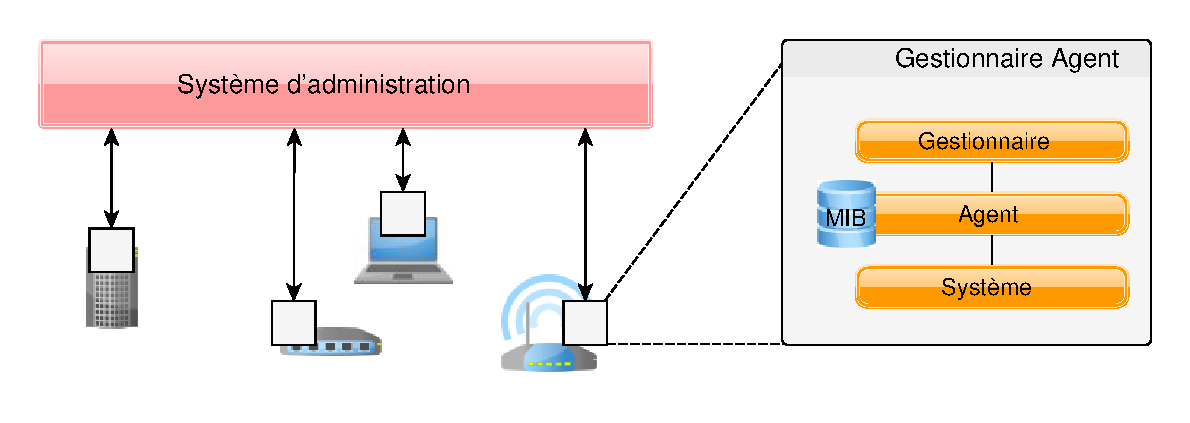
\includegraphics[width=.70\textwidth]{fig/rw-supervision-administration}
    \caption{Architecture d'un système classique d'administration}\label{fig:rw:supervision:administration}
\end{figure}

\subsubsection{Les données fournies par les agents}
Il existe plusieurs modèle de données dans le cadre des systèmes d'administrations. Le modèle le plus répandu reste la \textbf{structure hiérarchique}. La première apparition d'un tel modèle dans ce domaine remonte à la spécification de SNMP~\cite{IETF:SNMP} qui décrit le concept de \textit{Management Information Base} (MIB)~\cite{IETF:MIB}. Une \textit{MIB} est une base d'information où les données sont regroupées sous forme d'arbre. Chaque information possède un chemin unique (l'\textit{object identifier}) décrit par une suite de chiffres séparés de points.

Par exemple, \verb|1.3.6.1.2.1.2.2.1.2| est le chemin décrivant le nom d'une interface réseau sur un dispositif (par exemple \textit{eth0} sur un système Linux). Et le sous-arbre \verb|1.3.6.1.2| (MIB-II~\cite{IETF:MIB-II}) contient toutes les informations concernant les informations réseau du dispositif. Des catalogues répertorient désormais l'ensemble des \textit{MIB} existantes (standardisées ou non).

Les protocoles récents permettent aussi de manipuler des données de manière hiérarchiques sur les agents. Par exemple, dans le protocole TR-069, le modèle de données est décrit dans le rapport technique nommé \textit{TR-106}~\cite{BBF:tr106}. Dans le protocole UPnP-DM, le service de gestion de configuration (CMS)~\cite{UPnP:DMCMS} permet l'accès aux données. Dans ces derniers, le modèle de donnée est décrit comme un système de fichier. Les \textit{instances} sont assimilables à des dossiers, et les \textit{feuilles} sont assimilables à des fichiers. Les nœuds ont ainsi un nom et un chemin unique vers la racine \enquote{/}. 
\begin{figure}[ht]
    \centering
    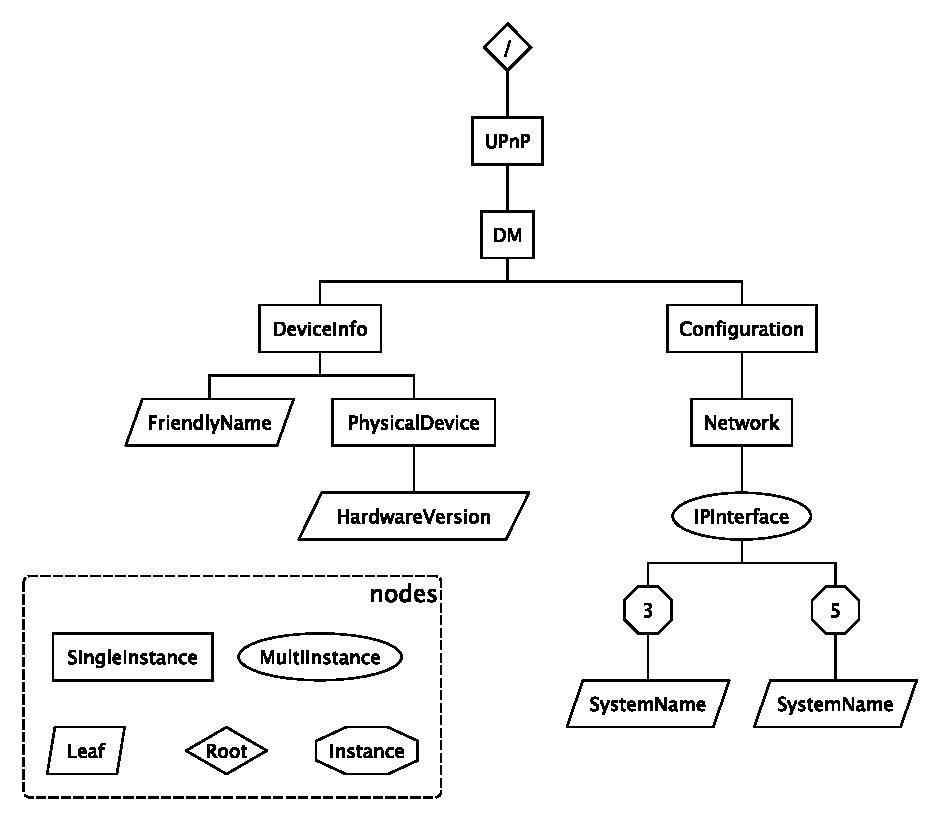
\includegraphics[width=.6\textwidth]{fig/rw-supervision-dmtree}
    \caption{Structure hiérarchique du modèle de données d'UPnP-DM}\label{fig:rw:supervision:dmtree}
\end{figure}

Un exemple de modèle de données de ce type de structure est présenté en figure~\ref{fig:rw:supervision:dmtree}. Une donnée est définie de manière unique, tout comme dans une \textit{MIB}, grâce à son chemin complet. Dans le vocabulaire du domaine de l'administration, cette donnée est appelée \textit{paramètre}. Le \textit{chemin} d'un paramètre est la concaténation des noms des nœuds qui le sépare de la racine, avec pour séparateur \enquote{/} dans UPnP ou \enquote{.} dans TR-069. L'implémentation de l'agent permet de créer et de remplir cette base d'information.

\begin{figure}[ht]
    \centering
    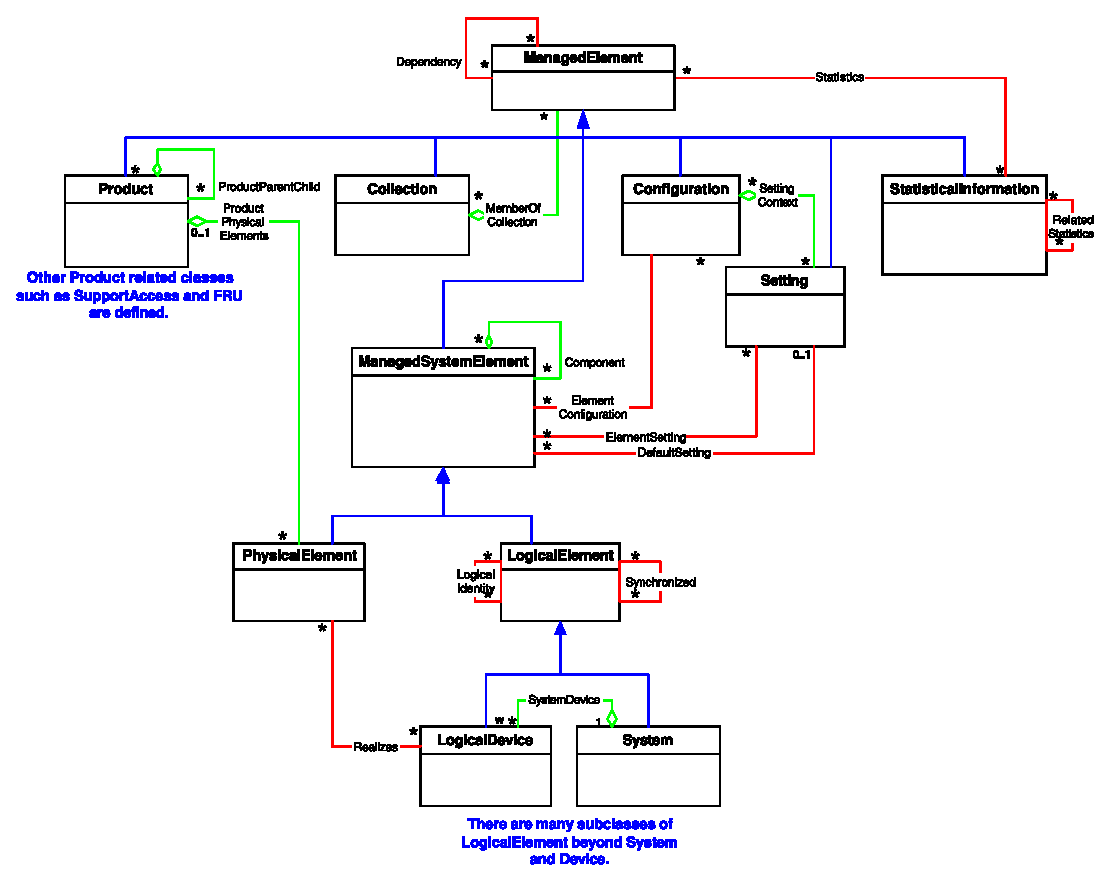
\includegraphics[width=.55\textwidth]{rw-supervision-cimcore}
    \caption{Modèle de classe de la partie \textit{Core} de \textit{CIM}}\label{fig:rw:supervision:cimcore}
\end{figure}
Toutefois, tous les modèles ne sont pas structurés sous forme de hiérarchie. Par exemple, la DMTF a adopté l'approche objet. En effet, dans les protocoles tels que WBEM~\cite{DMTF:WBEM} ou WS-MAN~\cite{DMTF:WS-MAN}, le modèle \textit{CIM} (\textit{Common Information Model})~\cite{DMTF:CIM} est décrit par un diagramme de classe UML comme présenté en figure~\ref{fig:rw:supervision:cimcore}. Ces protocoles sont notamment utilisés pour l'administration de web-services et applications entreprises. 

Plusieurs extensions standardisées existent pour modéliser les différents aspects des systèmes observés : Base de données, Dispositifs, Réseau, Sécurité, Utilisateur, Applications\dots{} Ainsi, le modèle de données est un modèle d'objet respectant l'ensemble des spécifications et des extensions. L'inconvénient majeur d'un tel choix reste la complexité de \textit{CIM} qui se trouve souvent réduite pour être applicable en pratique~\cite{Lopez:datacenter}.

Le système se compose ainsi de multiples agents qui sont une représentation de chaque objet. Les objets du système sont ainsi exposés à un service de gestion pour fournir plusieurs propriétés. Nous pouvons noter que ce principe reste le même pour l'administration de modules Java dans le protocole JMX~\cite{Sun:JMX} où des objets particuliers (les \textit{MBean}) sont exposés et peuvent être consultés et manipulés via ce protocole.

\subsubsection{Gestion de l'évolution des données}
Pour les différentes solutions présentées, les agents ont toujours trois modes principaux pour fournir des données :
\begin{itemize}
	\item[\textbf{Consultation indirecte}: ] Ce fonctionnement est le plus simple. La donnée est stockée dans une base d'information. Au moment de la consultation, l'agent lit directement dans la base et renvoie l'information.
	\item[\textbf{Consultation active}: ] Au moment de la consultation de la données via un primitive comme \enquote{\it get}, l'agent va effectuer le relevé actif de la donnée à la source. Ce relevé peut potentiellement prendre plus de temps qu'une simple lecture dans une base d'information.
	\item[\textbf{Événement}: ] La plupart des systèmes d'administrations supportent un mécanisme de \textit{publish}/\textit{subscribe} permettant de créer des canaux d'événements. La création d'événement se fait à partir du changement de valeur d'un paramètre ou à la création d'objets (ou de chemins).
\end{itemize}

Le problème majeur est que la consultation et les canaux d'événements sont deux approches et deux mécanismes différents qui sont rarement intégrés.

\subsubsection{Le gestionnaire global}
Dans l'architecture présentée en figure~\ref{fig:rw:supervision:administration}, de multiples agents fournissent différentes informations selon les modèles présentés dans la section précédente. Le système d'administration se connecte aux différents agents afin de les administrer. Il sert à la fois d'interface à l'utilisateur et d'infrastructure de collecte et d'analyse. Ainsi, il constitue la vue globale du système par l'intégration des données.

Il est important de noter que ce système peut ne pas être centralisé pour mieux amortir la charge en la présence de grandes quantités d'agents à administrer. Toutefois, pour l'administration de dispositifs des architectures centralisées peuvent suffire. Par exemple, pour l'administration de ses dispositifs, \textit{France Telecom} utilise un \textit{ACS} (\textit{Auto-configuration Server}, serveur d'administration en TR-069) centralisé. En effet, la fréquence d'émission des données en fonctionnement normal est lente (pour chaque dispositif, un rapport par jour typiquement). Pour les 10 millions d'équipements à gérer, une capacité de 500 réceptions par seconde côté serveur est suffisante. Cette capacité est atteinte sur des \textit{ACS} récents tels que \textit{EDGE}~\cite{Motorola:EDGE} de \textit{Motorola} sur des serveurs de puissance moyenne.

Toutefois, plus l'usage le requiert, plus ce type d'architecture ne peut supporter la charge des informations remontées. Plusieurs systèmes d'administrations proposent des architectures décentralisées (principalement hiérarchiques) pour la gestion à plus grande échelle~\cite{Kessis:management}. La hiérarchie peut se découper par lieu géographique, ou par domaine d'activité.

Nous venons de voir comment les systèmes d'administrations sont structurés et notamment comment ces systèmes modélisent leurs données. La section suivante présente les capacités de traitements de ce type de systèmes.

\subsection{Possibles traitements de données}
Que ce soit au niveau de l'agent comme au niveau du gestionnaire global, les données peuvent être traitées. Cette section détaille les différentes possibilités. Tout d'abord, nous voyons comment l'hétérogénéité des systèmes est traitée et comment l'intégration des multiples agents se fait. Par la suite, nous détaillons l'ajout de nœuds particuliers comme calcul de statistiques ou l'ajout de fonctions tierces.

\subsubsection{L'hétérogénéité par l'uniformisation des modèles}
La standardisation est un enjeux majeur pour les systèmes d'administrations à grande échelle. Comme présentés précédemment, la spécification les protocoles d'administrations des agents se fait autour de consortiums. Ainsi, l'hétérogénéité des systèmes est gérée par le respect des standards. Suivant les dispositifs observés, différents profils existent. Que ce soit pour les profils hiérarchiques ou à objet, des spécifications sont écrites pour décrire le modèle de données.

Le nombre de spécification augmente énormément pour essayer de limiter l'hétérogénéité. Par exemple, dans le cadre de \textit{TR-069}\footnote{Pour rappel, ce protocole est établit par un consortium d'opérateurs télécoms : le BBF}, il existe seulement 9 profils principaux. Mais lorsque les domaines d'activités s'élargissent le nombre d'entités devient difficile à contrôler, comme dans CIM où le nombre de spécifications est de 16\footnote{Sachant que les spécifications CIM sont bien plus complexes et possèdent plus d'entités.}, ou dans les MIB qui sont au nombre de 318 spécifiées par l'IETF.

Donc, la gestion de l'hétérogénéité se fait par la description de profils standardisés. Toutefois, la standardisation entraine des problèmes de complexité. Ce qui rend sa maîtrise plus difficile pour les utilisateurs.

\subsubsection{Intégration de sources}
L'avantage principal d'utiliser des modèles standards est l'intégration des sources de données. En effet, comme chacune des entités du système répond à un profil prédéfini, il est possible de faire l'union des données par catégorie pour avoir toutes les entités répondants aux différents profils. Ainsi, les données sont naturellement intégrées dans un modèle commun, ce qui permet aux concepteurs de systèmes d'observations de fournir des fonctions très avancées sans pour autant connaître l'instance du système. De plus, plusieurs protocoles et standards peuvent être utilisés dans un même système, comme l'a proposé WBEM, dans lequel des objets SNMP, JMX et autres sont intégrés à un modèle commun CIM.

Une fois les données accessibles à un niveau global, il devient possible de traiter ces données afin de les analyser, ou former des alertes. Pour cela, les systèmes d'administrations ne fournissent pas tous les mêmes capacités. Par défaut, la seule capacité que peut fournir l'agent est la récupération de son modèle de données (ou une sous-partie). Cependant, plusieurs systèmes permettent à l'utilisateur de définir des processus plus complexes pour permettre un traitement de plus haut niveau.

L'approche la plus utilisée est le \textit{scripting}. Le système d'observation fournit à l'utilisateur un langage \textbf{impératif} qui lui permet de définir des routines. Par exemple, EDGE~\cite{Motorola:EDGE} fournit une interface \textit{Javascript}, et l'\textit{ACS} d'\textit{Alcatel-Lucent} permet d'utiliser des programmes \textit{Python}. Ces routines peuvent par la suite être intégrées dans des réponses aux événements, ou dans des procédures de diagnostics ou encore de configuration.

Il est notable que les standards WBEM et WS-MAN définissent un langage \textbf{déclaratif} de manipulation de modèles CIM, le \textit{CQL} (\textit{CIM Query Language})~\cite{DMTF:CIM-QL}. Ce langage est très similaire à \textit{SQL} utilisé dans un cadre relationnel-objet. Dans sa spécification, il permet toutes les fonctionnalités de \textit{SQL} (sélection, projection, jointure, agrégation, imbrication de requêtes). Il est aussi utilisé afin de définir des filtres plus précis sur les événements (en remplacement du langage par défaut \textit{XPath}). Il est intéressant de noter que ce langage permet aussi la définition de \textit{politiques de gestions}, assimilables à des routines événements-condition-action. Toutefois, il reste peu implémenté dans la pratique.

\subsubsection{Sur l'agent : statistiques et extension}
Dans chacune des solutions présentées, il existe des parties du modèle des données consacrées à la présentation de statistiques. En effet, pour un paramètre dont la valeur représente une mesure, il peut être intéressant de fournir des extremums ou moyennes calculées à la volée. Plusieurs standardisations existent pour permettre un tel calcul principalement sur un échantillon précis ($N$ données) avec un ensemble fixé d'opérateurs.

Tous les modèles présentés sont extensibles à volonté par les constructeurs des dispositifs. Par exemple, sous UPnP-DM et TR-069, il est autorisé de rajouter des branches à l'arbre de données sous l'appellation \verb|X_{ORGANISATION}| (par exemple \verb|X_ORANGE_COM|). Ainsi, cela permet aux constructeurs de fournir des données non prévues dans les standards ou pour rajouter des fonctionnalités de traitement.

\subsection{Synthèse}
Le tableau~\ref{tab:rw:supervision:administration:synthese} résume l'ensemble de l'analyse pour les systèmes d'administrations. L'ensemble permet effectivement beaucoup de fonctionnalité pour les utilisateurs. Le choix d'approches principales à base de standard fait que ces systèmes sont actuellement très répandus pour gérer des systèmes de tous types. Ce qui en fait un excellent système pour collecter les données sur les ressources du système. Toutefois, le traitement des données est principalement faite dans un langage non-déclaratif. De plus, les canaux événementiels et la consultation des bases d'informations sont gérés dans des approches et mécanismes très différents. Ceci rend une observation intégrée difficile.


\begin{table}[!ht]
\criteretabDonnee
    {Principalement modèle \textbf{hiérarchique} sous forme de système de fichier. Quelques systèmes d'administration utilisent des modèles objets avec \textit{CIM}.}
    {Les différentes entités du systèmes sont des nœuds du modèle. Pas de contraintes ou d'inférences exprimables.}
    {Le dynamisme est géré par le mode d'accès. Certaines données peuvent être notifiables. Les mécanismes d'interrogations sont séparés.}
\criteretabTraitement
    {Instantanée et continue sur certaines données. Pas d'hybride possible vu que les procédés sont très séparés.}
    {Standardisation des modèles. Toutes les entités sont structurés dans le même formalisme. Intégration par union des données pour chaque profil.}
    {Appel de méthodes standardes pour récupérer un sous-arbre du modèle. Code impératif (scripting) principalement pour manipuler les données au niveau du gestionnaire. Utilisation de langage déclaratif (similaire SQL ou XPath) possible.}
    {Procédures à écrire en \textit{script}. Projection, sélection et union principalement. Certains nœuds particuliers permettent de calculer des statistiques.}
\criteretabAdaptabilite
    {Pas d'adaptation spécifique car les dispositifs doivent implémenter des standards.}
    {Pas de perspectives métiers en dehors de la sélection sur les branches du modèle.}
    {Nœuds particuliers pour le calcul. Fonctions métiers intégrées dans le gestionnaire.}
    {Très efficace et utilisé pour gérer des parcs de millions de dispositifs.}
\caption{Synthèse des systèmes d'administration}\label{tab:rw:supervision:administration:synthese}
\end{table}
\section{De l'importance de la supervision}\label{sec:intro:contexte}
%    Systèmes de plus en plus complexes

L'informatique a évolué de façon drastique au cours de ces dernières années. Grâce à l'amélioration des technologies de la micro-électronique, du réseau, et évidemment des techniques logicielles, il est désormais possible de concevoir des systèmes tels que :
\begin{itemize}
 \item Un réseau de capteurs. De nombreux micro-dispositifs autonomes, ou à durée de vie longue, capables de transmettre des informations sur une quantité physique sans fils. Ensembles, ils sont capables de créer un système de surveillance dans le cadre par exemple de l'agriculture de précision.
 \item Un environnement domestique intelligent. Grâce aux technologies sans-fil ou courant-porteur, des dispositifs sont capables de communiquer pour fournir des services de haut-niveaux. De tels services peuvent être  multimédia tels que le partage de flux vidéos ou la visiophonie. Mais aussi, ils peuvent être plus orienté sur l'amélioration du confort de vie de l'usager comme la gestion automatique des lumières ou encore l'assistance aux personnes handicapées.
 \item Un centre de traitement de données. Que ce soit pour virtualiser des services à très large échelle ou pour établir une ferme de calcul scientifique, la mise en relation de centaines d'équipements informatiques permet d'effectuer des traitements complexes.
\end{itemize}

%    Interactions nombreuses et volatiles
Ainsi, l'ordinateur personnel n'est plus qu'une partie des possibles interactions qu'un utilisateur quelconque peut faire avec l'informatique. Ces systèmes partagent la caractéristique principale suivante~: ces sont des dispositifs qui interagissent via un réseau pour fournir un service de haut niveau. Ces interactions sont nombreuses et potentiellement volatiles. Afin de mieux comprendre ces systèmes, il est nécessaire de les observer.

%    Établissement d'un diagnostic
La supervision d'un système est le processus en charge de collecter, traiter, et éventuellement stoquer les données relatives à un système pour en vérifier son bon fonctionnement. Cette surveillance peut s'effectuer en temps réel afin d'être pro-actif sur la réaction aux événements importants, ou par analyse a posteriori sur l'ensemble des données qui ont été collectées. Ainsi, lorsqu'un problème surgit sur un système, critique ou non, ce procédé est au cœur de la résolution de problèmes. En effet, si le traitement est en temps réel pourra détecter l'anomalie et pourra transmettre l'information à qui est capable d'y remédier (l'utilisateur ou système tiers). Sinon, il sera possible de retracer l'origine du problème par le parcours des données collectées afin d'établir un diagnostic.

%    Aide à l'administration
Enfin, la supervision est un outil central lors de l'administration du système. En effet, comme la surveillance passe aussi par la gestion de la configuration de chacun des dispositifs et services, il devient une base précieuse d'informations pour l'aide à la gestion du système car cela permet à l'administrateur d'avoir une vue détaillée du fonctionnement de son système.

Toutefois, le processus de surveillance doit être capable de répondre à la diversité et la grandissante complexité des systèmes informatiques. L'enjeu principal étant la capacité du système de supervision à s'adapter à l'hétérogénéité des systèmes, des dispositifs et des données. La section suivante présente plus en détail la problématique de cette thèse.
\section{Entrepôts de données}\label{sec:rw:supervision:warehouse}
Pilier de l'informatique décisionnelle (\textit{Business Intelligence}), l'approche par entrepôt de données (\textit{Data Warehouses}) est très réputé et grandement répendue. Son apport est originellement utilisé dans les applications pour entreprises. Toutefois sa capacité de traitement et ses outils d'analyses visuels ont permit son introduction dans d'autres cœurs de métiers tels que les réseaux~\cite{refneeded} ou l'agriculture~\cite{Abdullah:olap}. Cette architecture a été prévue pour permettre de fournir des outils d'analyses de données puissants. Pour cela, des procédés ont étés développés pour permettre de faire de l'intégration de données hétérogènes, ainsi que des structures d'entrepôts prêts à répondre aux besoins d'analyses.

Son impact dans le cadre de la supervision semble clair. En effet, puisque l'observation et la compréhension du système passe par son analyse, des outils sont nécessaires pour effectuer ces opérations. L'établissement de diagnostic nécessite effectivement le parcours des données pour mieux comprendre les causes d'un problème. De plus, sa structure permettant l'intégration de donnée est à considérer pour intégrer les sources de données auxquelles nous sommes confrontés.

Par la suite, cette section détaille en premier lieu l'architecture globale de la solution. Nous détaillerons ensuite comment l'intégration est faite via les processus \textit{ETL}. Ensuite nous décrirons les structures de données utilisées pour permettre différentes analyses. Enfin, nous présenterons brièvement quelques outils d'analyses pouvant raisonner sur les données.

\subsection{Architecture globale}
La définition fonctionnelle d'un entrepôt de donnée est \enquote{\it une collection de données orientées sujet, intégrées, non volatiles et historisées, organisées pour le support d’un processus d’aide à la décision}~\cite{Inmon:warehouse}. Au sens large, un entrepôt est une base de donnée avec une organisation qui s'oriente avant tout sur l'application finale (l'analyse) plutôt que sur l'intégrité des données, et qui refuse la suppression ou la modification de données afin de garder une trace.
\begin{figure}[ht]
	\centering
	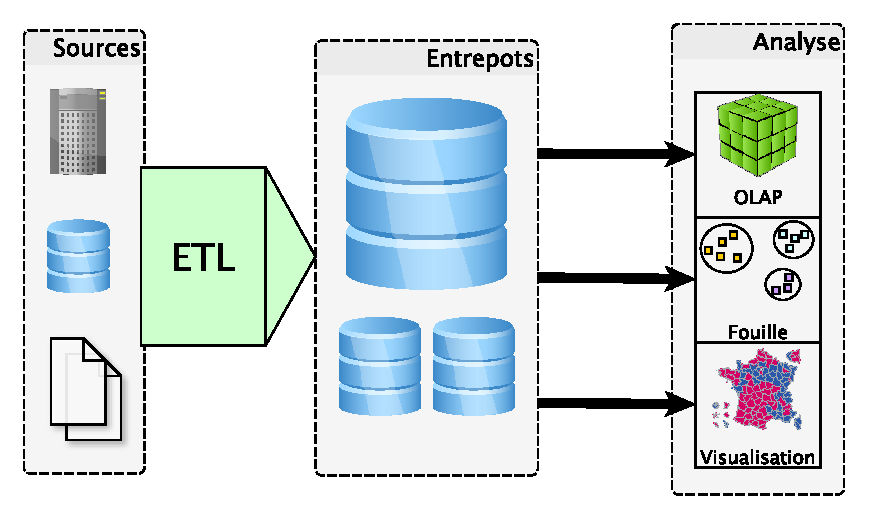
\includegraphics[width=0.75\textwidth]{rw-supervision-warehouses}
	\caption{Architecture globale d'une solution d'entrepôts de données}\label{fig:rw:supervision:warehouses}
\end{figure}
La figure~\ref{rw-supervision-warehouses} présente une architecture abstraite des approches à entrepots. Les données sources sont supposées être dans des bases de données opérationnelles au mieux, ou à l'intérieur de fichier brute, au pire. A partir de ce constat, il est acté que les sources sont donc hétérogènes autant en terme de syntaxe ou de sémantique.

Afin d'effectuer l'intégration des données à l'intérieur d'un (ou des) entrepôt(s), il faut traiter cette hétérogénéité et charger les données. Les processus \textit{ETL} ont été conçus pour cette tâche. Ces procédés sont découpés en trois phases : l'extraction (\textit{\textbf{E}xtract}), le traitement (\textit{\textbf{T}ransform}) et enfin le chargement (\textit{\textbf{L}oad}). Cet aspect sera détaillé en section~\ref{sec:rw:supervision:warehouse:etl}.

Par la suite, des outils d'analyses vont s'attacher aux entrepôts pour fournir les informations suffisantes à l'utilisateur pour qu'il puisse prendre une décision. Comme montré dans la définition des entrepôts, les bases de données sont conçus pour que ces outils d'analyses puissent effectuer leurs calculs nativement. La structure interne des entrepôts aura donc un impact sur la capacité des outils d'analyse.

\subsection{L'entrepôt et ses capacités}\label{sec:rw:supervision:warehouse:warehouse}
Les dépots de données ont pour but de stocker toutes les données relatives à un système. Son système de gestion est très souvent fait par un SGFD relationnel\footnote{Il est évident que des systèmes de gestion dédiés soient choisis pour des critères de performances}. C'est sa structure et ses opérations qui vont permettre une analyse pertinente.

Le cadre le plus récurrent pour les entrepôts de données est le traitement OLAP (\textit{Online Analytical Processing}). 
\subsubsection{OLAP}
Le terme \textit{OLAP} a été d'abord défini en 1993 par le père du modèle relationnel, Edgar Codd, dans~\cite{Codd:olap}. Sa caractérisation est le fait de permettre le support \textit{d'analyse de données multidimensionnelles}. En effet, il apparait qu'une donnée représente un point dans un espace à plusieurs dimensions. L'exemple le plus standard dans ce domaine reste la gestion de vente pour une entreprise. La vente est un point dans l'espace $(Magasin, Produit, Temps)$ et sa valeur sera le prix (et/ou la quantité). L'analyse de ces données sur ces trois critères requiert des capacités spécifiques pour que l'analyse soit pertinente.

En 1995, les premiers concepts d'opérations multidimensionnelles arrivent avec le \textbf{cube}~\cite{Gray:cube}. Les dimensions doivent être définies de manière hiérarchique. Par exemple, un magasin (lieu) est située dans une ville, elle-même située dans un département, elle même située dans une région etc.. Par la suite, le traitement sur les données en elle-même va être centré sur la capacité à faire un agrégat. Dans notre cas, il est potentiellement intéressant de voir les résultats de vente par départements. Une somme est ainsi faite sur tous les résultats de chaque département.

L'hypercube \textit{OLAP} est la représentation des données multidimensionnelles. Dans notre cas, cela va être un vrai cube à trois dimensions, les magasins, les produits, et le temps. Au début de l'analyse les dimensions sont discrétisé à leur plus haut niveau hiérarchique.
\begin{figure}[ht]
	\centering
	\TODO{}
	\caption{Représentation d'un cube \textit{OLAP} de trois dimensions, $(Magasin, Produit, Temps)$}
\end{figure}
Cela forme un découpage du cube en autres cubies. Chacun de ces cubies contient la valeur d'un ou plusieurs agrégats choisis par l'utilisateur (ici, \textit{SUM}). Il est important de dire que l'utilisateur ne pourra pas que rarement exploiter correctement les $n$ dimensions de l'hypercube, car la représentation classique des données est sous forme de tableaux (donc 2 dimensions). Plusieurs opérations génériques existent sur ce cube pour que l'utilisateur puisse l'exploiter.

\subsubsection{Opérations du cube}
\begin{itemize}
	\item[\textbf{Slice}] : Découpage du cube selon une des dimensions. Cela permet de retirer la complexité de l'analyse et de ne sélectionner qu'une partie des données selon un critère dimensionnel. Exemple : \textit{slice} du cube sur \textit{temps = 2012}.
	\item[\textbf{Dice}] : Extraction d'un sous-cube. Similaire à \textit{slice}, toutefois, la complexité n'est pas spécifiquement réduite car le nombre de dimension n'a pas changé. Exemple : extraction du cube pour les magasins \textit{La Boite à Musique} et \textit{Michel Musique}.
	\item[\textbf{Drill-down}] : Permet de faire la navigation à l'intérieur d'une dimension. Par exemple, le \textit{drill-down} du cube sur l'année \textit{2011} va couvrir la dimension du temps du 1er janvier 2011 jusqu'au 31 décembre 2011, en découpant la dimension par mois. Un autre \textit{drill-down} découpera en fonction des jours.
	\item[\textbf{Drill-up}] : Opération inverse de \textit{drill-down}. Ici, l'analyste remonte dans l'abstraction de la dimension de navigation (en passant d'une granularité par \textit{guitares} à \textit{instruments à cordes}).
	\item[\textbf{Pivot}] : Changement de perspective du cube. Jusqu'ici, le cube était représenté avec comme axes principaux $(Magasin, Produit)$. Le rapport à l'utilisateur se fait donc par ce biais principalement. Le pivot permet de tourner le cube pour changer ces axes.
\end{itemize}
L'opération \textit{roll-up} permet de calculer tous les agrégats à partir d'une ou plusieurs dimensions. Pour un tableau cela implique de calculer les agrégats par ligne, par colonne et au total. Ces outils sont extrèmement puissant en terme de pouvoir d'analyse.

D'un point de vue performance, les concepts de systèmes \textit{OLAP} optimisent les performances des manipulations sur le cube ainsi que les agrégats. Toutefois, si les requêtes sont trop complexes, les analyses peuvent prendre plusieurs minutes (ou pire, plusieurs heures).

\subsubsection{La visualisation : un domaine à part entière}


\subsubsection{Data Mart}

\subsection{L'intégration par ETL}\label{sec:rw:supervision:warehouse:etl}
\subsection{Synthèse}
\section{Gestion de flux de données}\label{sec:rw:supervision:datastream}
Devant la multiplication des applications à base de flux de données telles que : la gestion des données de capteurs ou la surveillance réseau, les \textit{Systèmes de Gestion de Flux de Données} (\textit{SGFD}) ont été conçus pour mieux maîtriser les données de ce type~\cite{Madden:tag, Yao:cougar, Cranor:gigascope}. L'idée principale est de permettre l'interrogation des flux de données via un langage déclaratif (tout comme le \textit{SQL}) avec un grand pouvoir d'expression.

La gestion de flux est le socle fondamental des systèmes capables de traiter les événements. Les travaux récents sur les \textit{CEP} temps réel (\textit{Complex Event Processing}) permettant de faire de la détection d'événements complexes~\cite{Brenna:cayuga} peuvent être vu au final comme une extension des SGFD avec des opérateurs spécifiques et optimisés. L'expression des motifs d'événements pourront être complexes à écrire et à évaluer mais le concept reste d'évaluer des requêtes continues sur des flux de manière déclaratives. Cet aspect conforte nos besoins en terme d'extensibilité du système d'observation.

\subsection{Approche des SGFD}
Un flux de données est une série de données qui s'accumulent au fur et à mesure du temps~\cite{Golab:issues}. De façon générale, un flux n'est pas considéré comme régulier, par exemple \enquote{\it une donnée toutes les 5 secondes}. L'idée de faire une interrogation sur ces flux de données au sens \enquote{gestion de base de données} du terme n'a pas de sens, car il y aurait confusion entre les modes d'interrogations continues et instantanées présentés en section~\ref{sec:intro:problematique}. En effet, le paradigme des requêtes est fondamentalement différent, car les requêtes sont de longue durée et persistantes~\cite{Chen:niagaracq} comme illustré dans la figure~\ref{fig:rw:supervision:sgbd-sgfd}. Nous détaillons ici les différences conceptuelles entre SGBD et SGFD.
\begin{figure}[ht]
    \centering
    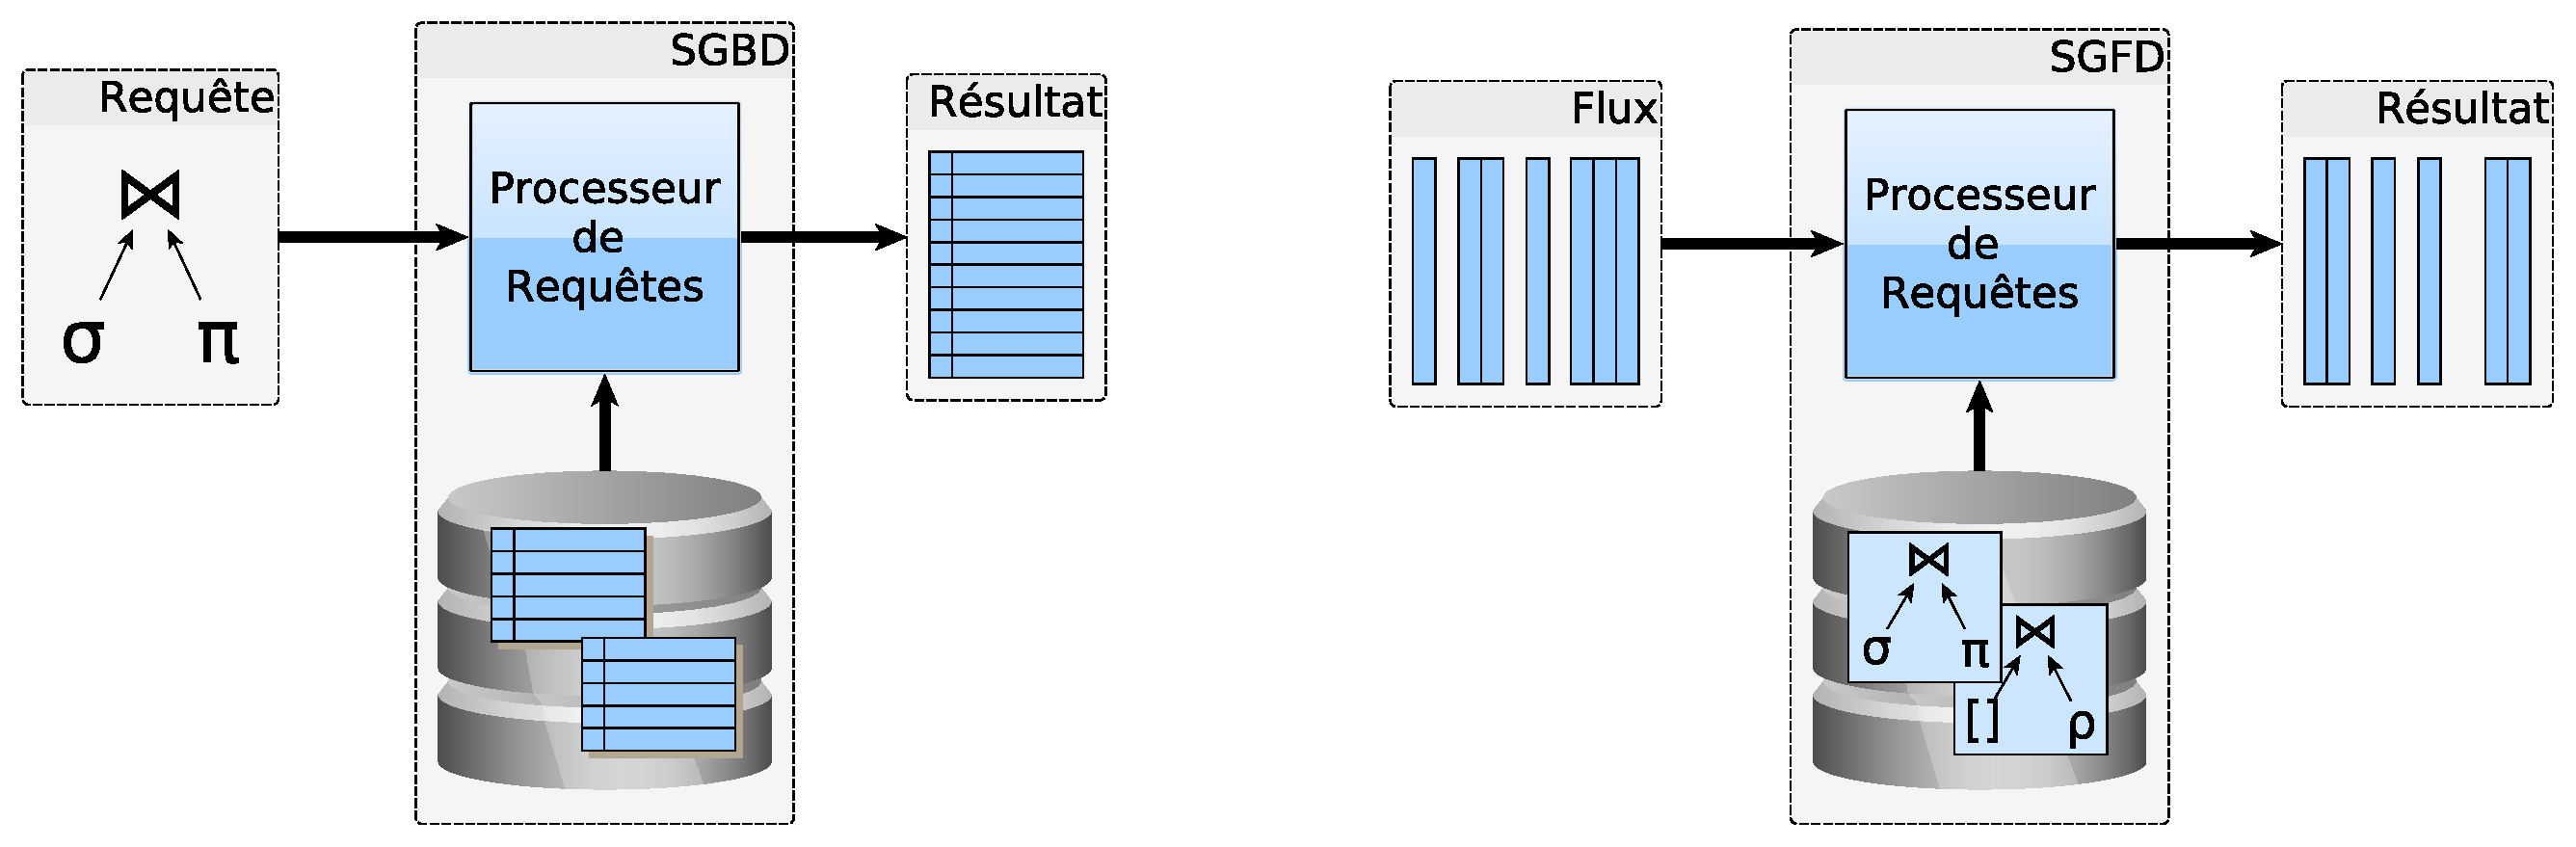
\includegraphics[width=0.75\textwidth]{rw-supervision-sgbd-sgfd}
    \caption{SGBD : Requêtes transitoires, Données persistantes vs SGFD : Données transitoires, Requêtes persistantes~\protect\cite{Gurgen:sstreamware}}\label{fig:rw:supervision:sgbd-sgfd}
\end{figure}

\begin{itemize}
    \item[\textbf{Base de données}] : Une requête est une question posée sur un ensemble de relations figées et persistantes (principe transactionnel). La réponse est un ensemble de n-uplets. Une fois la requête traitée elle n'existe plus.
    \item[\textbf{Flux de données}] : Une requête est un ensemble d'opérateurs considéré comme persistant. Le ou les flux de données sont appliqués sur cet ensemble d'opérateurs pour en produire un nouveau flux. La particularité d'un flux de données est qu'une fois la donnée \textit{consommée}, elle n'est plus considérée comme présente dans le flux d'entrée. Les données fournies en entrée de la requête sont  transitoires.
\end{itemize}

Ainsi, le terme \textit{requête} a un tout autre sens. Toutefois, beaucoup de concepts sont applicables dans ce contexte. En effet, plusieurs éléments du modèle relationnel sont appliqués dans ce domaine~\cite{Arasu:semantic}. Historiquement, les premières requêtes continues~\cite{Terry:tapestry} étaient une exécution périodique de requêtes \textit{SQL}. Le traitement était entièrement basé sur les opérateurs du modèle relationnel standard. Par la suite, les modèles ont évolué pour supporter le dynamisme propre aux flux.

\subsection{Intérêt pour l'observation de systèmes}
La gestion de flux de données a été créée pour mieux gérer le dynamisme des données. Le résultat montre qu'effectivement, il est possible de faire des requêtes continues sur des flux de données de manière déclarative et avec des performances très efficaces, ce qui correspond à nos exigences pour un système d'observation.

Toutefois, la complexité qui en ressort comparé à celle de l'algèbre relationnelle est plus importante. De plus, les données sont considérées comme uniquement volatiles. Pour notre problématique, il est nécessaire de pouvoir gérer les données persistantes et les requêtes instantanées. Cette approche semble être la plus proche de notre objectif. Ainsi, nous consacrons le chapitre~\ref{chap:rw:sgfd} à son analyse détaillée.

\begin{table}[!ht]
\criteretabDonnee
    {Modèle dérivé du relationnel, mais où le contenu est variable dans le temps.}
    {Ensemble de sources indépendantes sauf représentation ad hoc.}
    {Toutes les données sont dynamiques et événementielles a priori.}
\criteretabTraitement
    {Continue.}
    {Il est supposé que chaque source produit un flux de données. Le fait de traiter ces flux participe à l'intégration de sources.}
    {Langages de requêtes similaires aux SQL supportant la dynamique des données}
    {À un instant donné, les opérateurs sont semblables au relationnel. L'expressivité du support de l'évolution des données reste inconnue encore.}
\criteretabAdaptabilite
    {Création de source pour fournir les flux de données. Comme il n'y a pas de schéma conceptuel, l'adaptation est l'écriture de requêtes continues.}
    {Pas de perspectives métiers.}
    {Les sources et puits sont en général adaptés par les utilisateurs. Un développement peut être fait dessus, mais il est rarement possible de rajouter des opérateurs.}
    {Très rapide, car la latence de traitement doit être contrôlée pour supporter des hauts débits.}
\caption{Synthèse des systèmes de gestion de flux de données}\label{tab:rw:supervision:sgfd:synthese}
\end{table}

\section{Conclusion}
Ce chapitre a dressé un état de l'art des différents systèmes capables d'offrir une solution générique de supervision. Il en ressort qu'aucun système ne supporte entièrement les critères de qualité que nous nous sommes fixés. Le tableau~\ref{tab:rw:supervision:bilan} résume les 11 points d'analyse en colorant les différentes points suivant leurs conformités. 

\begin{sidewaystable}[ht]
\centering
\begin{tabular}{@{{\vrule width 1pt}\ \ }>{\raggedleft}m{3cm}@{\ \ {\vrule width 1pt}\ \ }M{4.2cm}|M{4.2cm}|M{4.2cm}|M{4.2cm}@{\ \ {\vrule width 1pt}}} \bottomrule
\head Critère & \head Système d'administration & \head Gestion de contexte & \head Entrepôts de données & \head Gestion de flux de données \\  \toprule \bottomrule
\critereAA & Hiérarchique & Triplets & Relationnel & Relationnel dérivé \\ \hline
\critereAB & \meh Structure hiérarchique sans contraintes & \good Ontologies & \good Modèle relationnel normalisé & \bad Pas de structure \\ \hline
\critereAC & \meh Notifications & \bad Ajout du temps en propriété & \meh CDC & \good Flux natif \\ \toprule \bottomrule
\critereBA & \meh Instantanée, continu en ad-hoc & \bad Instantané principalement & \meh Instantané. ETL en pseudo-continu & \bad Continu uniquement \\ \hline
\critereBB & \good Standardisation, union de modèles & \meh Fusion d'ontologies non standardes & \good Processus ETL (complexe) & \good Union et jointures de flux \\ \hline
\critereBC & \bad Impératif principalement & \good Logique & \meh Déclaratif (SQL) et Procédural (ETL) & \good Déclaratif principalement\\ \hline
\critereBD & \meh Procédures à écrire soi-même & \good Logique du premier ordre & \good Relationnel multidimensionnel et Algorithmie dédiée & \meh Relationnel avec support du dynamisme\\ \toprule \bottomrule
\critereCA & \good Support des standards & \meh Spécification longue des domaines & \bad Spécification du schéma, des ETL, autre (complexe) & \good Écriture de requêtes \\ \hline
\critereCB & \bad Aucune & \good Séparation par les domaines & \good Données multidimensionnelles & \bad Aucune \\ \hline
\critereCC & \good Modèle extensible, fonctions métiers dans le gestionnaire & \meh Capteurs virtuels & \good Opérateurs ETL, procédures SQL, algorithmes & \meh Sources et puits mais pas les opérateurs  \\ \hline
\critereCD & \good Large échelle & \bad Complexité très haute & \meh Réactivité lente, Support de grande quantité & \good Support de haut débits\\ \toprule 
\end{tabular}
\caption{Récapitulatif de l'état de l'art des systèmes génériques de supervision}\label{tab:rw:supervision:bilan}
\end{sidewaystable}
Il en ressort que les systèmes d'administrations sont avant tout des systèmes qui fonctionnent grâce au support des standards et à leur simplicité d'implémentation. L'architecture avec gestionnaire adaptable grâce à des langages impératifs permets une grande flexibilité pour s'adapter aux cas d'usages. De son côté, l'informatique contextuelle fournit des outils permettant de modéliser et manipuler proprement les concepts du système grâce aux ontologies et aux raisonnements logiques. Il en sort une claire séparation des domaines de compétences. Les entrepôts de données quant à eux se distinguent par des capacités d'analyses très poussées, ainsi qu'un procédé d'intégration, très complexe et lourd malheureusement, mais très complet. Enfin, la gestion de flux de données est une base solide pour gérer les données dynamiques. L'intégration et l'adaptation au système étant fait entièrement de manière déclarative en fait une solution performante et viable.

À la vue de l'état de l'art, voici les points qui vont être critique sur notre établissement de notre contribution :
\begin{itemize}
    \item La gestion de flux est un bon socle pour gérer les données dynamique grâce aux requêtes continues.
    \item Elle ne suffit pas pour constituer un système d'observation complet, notamment à l'absence de modèle de description et de requêtes instantanées.
    \item Les entrepôts et bases de données sont capables de répondre aux requêtes instantanées.
    \item Les ETL sont trop complexes à manipuler pour intégrer les données, alors que les SGFD sont plus déclaratifs.
\end{itemize}
Il devient clair que les systèmes de gestions de flux de données forment un bon candidat comme fondation pour un architecture d'observation de système. Il nous faut donc approfondir l'état de l'art technique sur ce domaine pour modeler notre contribution. Le point majeur sera d'apporter les capacités des systèmes de gestions de données relationnels. En effet, en apportant le support persistant à la gestion de flux de données, en clarifiant et augmentant son langage, nous aurons un outil qui sera plus apte à répondre à notre problématique. Ainsi, l'héritage du relationnel permettra une structure sémantique correcte, ainsi que des capacités d'analyses plus évoluées. Enfin et surtout, les données serait intégrés malgré leur hétérogénéité profonde. Le chapitre suivant détaille l'état de l'art technique de la gestion de flux de données afin de pouvoir effectuer ces améliorations.
